\documentclass[../main.tex]{subfiles}
\graphicspath{{\subfix{../../images/}}}

\begin{document}

\subsection{IP addresses}

IP stands for the Internet Protocol, and IP addresses are like street addresses; in the sense that they represent locations on a network. There are 2 main types, IPv4 and IPv6 addresses.

\begin{figure}[h]
    \centering
    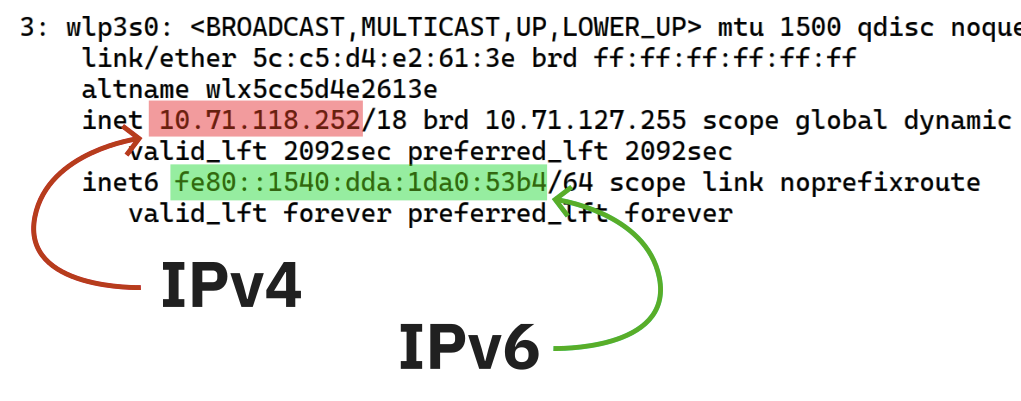
\includegraphics[width=0.7\textwidth]{ip_addresses}
    \caption{Output from the Linux {\mono ip} utility, showing IPv4 and V6 addresses}
\end{figure}

\paragraph{IPv4 Addresses}

Are \textbf{32-bit values} represented as 4 3-digit numbers with dots between them, like {\mono 192.168.0.1} with each value ranging between 0-255. There are 2 tyes of IP addresses, \emph{Public} and \emph{Private} IP addresses.

\begin{figure}[h]
    \centering
    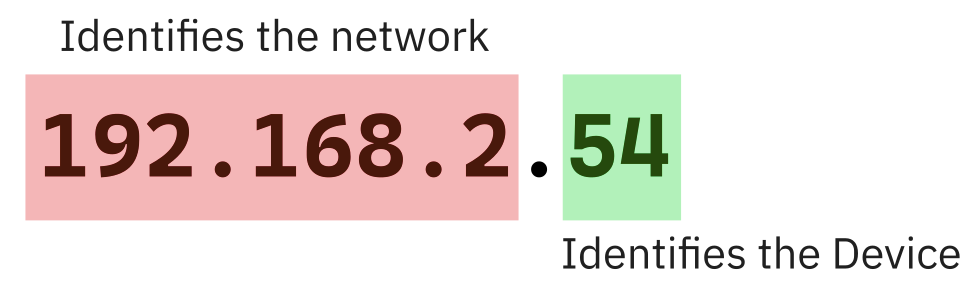
\includegraphics[width=0.7\textwidth]{ipaddr_breakdown}
    \caption{The two components of an IPv4 address}
    \label{fig:ipaddr_breakdown}
\end{figure}

Figure \ref{fig:ipaddr_breakdown} shows the two main components of IPv4 addresses; the first component determines the network itself, and the second component determines the device on the network uniquely.

In terms of private and public networks it will be covered more in \textbf{Chapter 4} and later sections about NATs.

\paragraph{Public IPv4 Addresses}

These IP addresses denote the location of your home router or other routers on the public internet. All web servers, like the one in our school or your personal router has a public IP address accessible by everybody\footnote{although they do not necessarily respond with data all the time}.

The only rule they must follow is that their addresses cannot be in the range of \hyperref[tab:private_ip_classes]{private IP addresses}.

\paragraph{Private IPv4 Addresses}

Private IP addresses are like public IP addresses, but instead of it being publicly accessible to everybody on the internet, they are only accessible to users connected to a private network, like a phone hotspot or the network created by your router. Every device on, say, your home network like your phone or your mom's work laptop have a private IP. These addresses are then mapped to public IP addresses through NATs (Network Address Translators); more details in section \ref{2:sec:nats}.

In the IPv4 address range, addresses are reserved for private networks to use, and they are:\footnote{Taken from \url{https://www.geeksforgeeks.org/private-ip-addresses-in-networking/}}

\begin{figure}[ht]
    \centering
    \begin{tabular}{ |c|c|c| }
        \hline
        \textbf{Class} & \textbf{IP Range} & \textbf{Most typically seen in} \\ \hline 
        A & {\mono 10.0.0.0} to {\mono 10.255.255.255}     & Large networks \\ \hline
        B & {\mono 172.16.0.0} to {\mono 172.31.255.255}   & Medium-sized networks \\ \hline 
        C & {\mono 192.168.0.0} to {\mono 192.168.255.255} & Small networks \\
        \hline
    \end{tabular}
    \caption{Table of private IP classes}
    \label{tab:private_ip_classes}
\end{figure}

Note that you do not need to memorize the class letters nor the exact ranges, you just need to identify them, especially the most common one, class C which is between {\mono 192.168.0.0} to {\mono 192.168.255.255}.

These private IPs belong in a local network, where devices in the same approximate geographical location are connected to a router.

\subsubsection{Dynamic IP assignment}

\subsubsection{Static IP assignment}

\subsection{MAC addresses}

\subsubsection{Universally Administered}

\subsubsection{Locally Administered}

\end{document}
